\documentclass[t,xcolor=pdftex,dvipsnames,table]{beamer}
\usepackage[]{graphicx}\usepackage[]{color}
%% maxwidth is the original width if it is less than linewidth
%% otherwise use linewidth (to make sure the graphics do not exceed the margin)
\makeatletter
\def\maxwidth{ %
  \ifdim\Gin@nat@width>\linewidth
    \linewidth
  \else
    \Gin@nat@width
  \fi
}
\makeatother

\definecolor{fgcolor}{rgb}{0.345, 0.345, 0.345}
\newcommand{\hlnum}[1]{\textcolor[rgb]{0.686,0.059,0.569}{#1}}%
\newcommand{\hlstr}[1]{\textcolor[rgb]{0.192,0.494,0.8}{#1}}%
\newcommand{\hlcom}[1]{\textcolor[rgb]{0.678,0.584,0.686}{\textit{#1}}}%
\newcommand{\hlopt}[1]{\textcolor[rgb]{0,0,0}{#1}}%
\newcommand{\hlstd}[1]{\textcolor[rgb]{0.345,0.345,0.345}{#1}}%
\newcommand{\hlkwa}[1]{\textcolor[rgb]{0.161,0.373,0.58}{\textbf{#1}}}%
\newcommand{\hlkwb}[1]{\textcolor[rgb]{0.69,0.353,0.396}{#1}}%
\newcommand{\hlkwc}[1]{\textcolor[rgb]{0.333,0.667,0.333}{#1}}%
\newcommand{\hlkwd}[1]{\textcolor[rgb]{0.737,0.353,0.396}{\textbf{#1}}}%
\let\hlipl\hlkwb

\usepackage{framed}
\makeatletter
\newenvironment{kframe}{%
 \def\at@end@of@kframe{}%
 \ifinner\ifhmode%
  \def\at@end@of@kframe{\end{minipage}}%
  \begin{minipage}{\columnwidth}%
 \fi\fi%
 \def\FrameCommand##1{\hskip\@totalleftmargin \hskip-\fboxsep
 \colorbox{shadecolor}{##1}\hskip-\fboxsep
     % There is no \\@totalrightmargin, so:
     \hskip-\linewidth \hskip-\@totalleftmargin \hskip\columnwidth}%
 \MakeFramed {\advance\hsize-\width
   \@totalleftmargin\z@ \linewidth\hsize
   \@setminipage}}%
 {\par\unskip\endMakeFramed%
 \at@end@of@kframe}
\makeatother

\definecolor{shadecolor}{rgb}{.97, .97, .97}
\definecolor{messagecolor}{rgb}{0, 0, 0}
\definecolor{warningcolor}{rgb}{1, 0, 1}
\definecolor{errorcolor}{rgb}{1, 0, 0}
\newenvironment{knitrout}{}{} % an empty environment to be redefined in TeX

\usepackage{alltt}
\newcommand{\SweaveOpts}[1]{}  % do not interfere with LaTeX
\newcommand{\SweaveInput}[1]{} % because they are not real TeX commands
\newcommand{\Sexpr}[1]{}       % will only be parsed by R


%\documentclass[handout,t,xcolor=pdftex,dvipsnames,table]{beamer}  % For handout
\mode<presentation>{
\useoutertheme[subsection=false]{miniframes}
%\beamertemplatenavigationsymbolsempty
\usecolortheme{custom}
\usefonttheme[onlymath]{serif}
\setbeamercovered{invisible}
%\setbeamertemplate{navigation symbols}{}
%\setbeamertemplate{mini frames}{}  % Old one
% Comment out this line to give the header
% \setbeamertemplate{headline}[default]
\setbeamertemplate{caption}[numbered]
%\setbeamertemplate{itemize items}[circle] 
\setbeamertemplate{frametitle continuation}{\frametitle{\color{white}Title}}  % So no tile on subsequent frames, from [allowframebreaks]

%%% CUSTOMISING NAVIATION %%%%
%This customises the navigation to be thin width and just have section headings (not subsections). 
\setbeamertemplate{headline}{%
\leavevmode%
  \hbox{%
    \begin{beamercolorbox}[wd=\paperwidth,ht=2.5ex,dp=1.125ex]{palette tertiary}%   % Tertiary colour is blue
    \insertsectionnavigationhorizontal{\paperwidth}{}{\hskip0pt plus1filll}
    \end{beamercolorbox}%
}}}

\RequirePackage{marvosym}

%%% INCLUDING SOLUTIONS %%%%
%% You can incorporate both questions and solutions in the 
%% same document.  Solutions can be included between the 
%% commands \begin{soln} and \end{soln}
%% To generate a pdf with only the questions uncomment:
%\excludecomment{soln}
\usepackage{comment}
\specialcomment{soln}{\begingroup \vspace{1mm} \sl}{ \leavevmode \endgroup}

%%%% DETAILS FOR PART 1 TITLE PAGE (OLD) %%%%
%\title{\large Part2 - Probability \& Distribution Theory} 
%\subtitle{} 
%\author{\copyright Dr Di Warren 2016} 
%\date{MATH1005 - Statistics}
% \colorlet{Faculty}{Arts}
%\colorlet{Faculty}{MasterBrandRed} % This is only needed if the notes are used for different faculties.
%\colorlet{FacultyText}{White}
% Defines the color of the text used on the title page and ``blocks''
% White for Business; TitlePageBlack for Arts, Pharmacy and Science
%\definecolor{CoolBlack}{rgb}{0.0, 0.18, 0.39}

%%%% DETAILS FOR FULL COURSE TITLE PAGE %%%%
\title{\Huge STATISTICS} 
\subtitle{} 
\author{\copyright University of Sydney 2017 (Di Warren)} 
\date{MATH1005}
% \colorlet{Faculty}{Arts}
\colorlet{Faculty}{MasterBrandRed} % This is only needed if the notes are used for different faculties.
\colorlet{FacultyText}{White}
% Defines the color of the text used on the title page and ``blocks''
% White for Business; TitlePageBlack for Arts, Pharmacy and Science
\definecolor{CoolBlack}{rgb}{0.0, 0.18, 0.39}

%%%% PACKAGES %%%%
\usepackage{multirow}
\usepackage{fancybox}
\usepackage[english]{babel}
\usepackage[utf8]{inputenc}
\usepackage{bm}
\usepackage{array}
\usepackage{booktabs}
\usepackage{tikz}
\usetikzlibrary{matrix,arrows,decorations.pathmorphing}
\usepackage{verbatim}
\usepackage{pgf,pgfsys,pgffor}
\usepackage{pgfplots}
\pgfplotsset{compat=1.3} %Recommended as of Pgfplots 1.3 - necessary?
\usetikzlibrary{decorations.pathreplacing,calc}
\usetikzlibrary{shapes, backgrounds}   % For Venn diagrams
\def \setA{ (0,0) circle (1cm) }
\def \setB{ (1.5,0) circle (1cm) }
\def \setC{ (0.6,1.5) circle (1cm) }
\def \setO{ (-2, -1.5) rectangle (3.5, 2.75) }
\tikzstyle{every picture}+=[remember picture]
\tikzstyle{na} = [baseline=-.5ex]
\usepackage{listings}  %Added by Di for adding R code

%\AtBeginSection[]
%{
%   \begin{frame}
 %      \frametitle{Outline}
 %      \tableofcontents[currentsection]
%   \end{frame}
%}  %This seems overkill for weekly lecture slides.

%\AtBeginSection[]
%{
%  \begin{frame}
% \frametitle{Contents}
%  \tiny{\tableofcontents[currentsection]}
%  \end{frame}
%}
%\useoutertheme{infolines} % Just lists current section in navigation at top, nice but limiting?

%%%% TITLE PAGE AND CONTENTS AT BEGINNING OF EACH TOPIC %%%%

\RequirePackage{ifthen} % package required
\newboolean{sectiontoc}
\setboolean{sectiontoc}{true} %default to true

\AtBeginSection[]
{
\begin{frame}[plain]
\vspace{60pt}
\begin{center}
\Huge{{\textcolor{MasterBrandBlue} \insertsection}}
\end{center}
\begin{tikzpicture}[scale=0.54]
%\hspace{-12pt}
%% Big Rectangle
\fill[MasterBrandRed] (0,14) -- (20,14) -- (20,15) -- (0,15);

%\draw (1,14.5) node [anchor = west] {\textcolor{MasterBrandBlue}{\Huge{\insertsection}}}; Overlays box with title, but long titles drop off the page
\end{tikzpicture} 
\end{frame}

%%%%%WORKING VERSION OF TOC%%%%%
%\begin{frame}
%   \frametitle{Outline}
%  \tableofcontents[currentsection, sectionstyle=show/hide, subsectionstyle=show/show/hide]
%  \end{frame}
%}

%%%%%2 VERSIONS - WITH AND WITHOUT TOC%%%%%
  \ifthenelse{\boolean{sectiontoc}}{
    \begin{frame}
  \frametitle{Outline}
  \tableofcontents[currentsection, sectionstyle=show/hide, subsectionstyle=show/show/hide]
 \end{frame}
  }
}
%%%%%This doesnt seem to work?%%%%
\newcommand{\toclesssection}[1]{
  \setboolean{sectiontoc}{false}
  %\section{#1}
  \setboolean{sectiontoc}{true}
}


% PDF settings
%\hypersetup{%
%  pdftitle={\inserttitle \insertsubtitle},%
%  pdfauthor={Di Warren},%
%	pdfsubject={},%
%	pdfkeywords={}%   
%	 }

%%%%  HELPFUL MACROS %%%%
\newcommand{\ud}{\mathrm{d}}
\newcommand{\var}{\mathrm{var}}
\newcommand{\ep}{\varepsilon}
\newcommand{\cov}{\mathrm{cov}}
\newcommand{\tr}{\mathrm{tr}}
\newcommand{\MSE}{\mathrm{MSE}}
\newcommand{\rank}{\mathrm{rank}}
\newcommand{\Bias}{\mathrm{Bias}}
\newcommand{\dei}{\partial}
\newcommand{\E}{\mathbb{E}}
\newcommand{\N}{\mathcal{N}}
\newcommand{\bbR}{\mathbb{R}}
\newcommand{\V}{\mathbb{V}}
\newcommand{\betahat}{\hat{\beta}}
\newcommand{\CLRM}{$\mathbf{y} = X\bm{\beta} + \bm{\ep}$}

%%%% LOGO FOR SLIDES %%%%
\logo{\vspace{79mm}
\includegraphics[height=0.9cm]{../images/sydney.pdf}}

%%%% ADD PAGE NUMBER %%%%
\setbeamertemplate{sidebar right}{}
\setbeamertemplate{footline}{%
\hfill\usebeamertemplate***{navigation symbols}
\hspace{1cm}\insertframenumber{}/\inserttotalframenumber}

%%%% BEGIN CONTENT %%%


\begin{document}



%%%% TOPIC4 %%%%
\section[4]{Topic4: Probability, Random Variables and Distributions}

\subsection[]{Example: Coin Tossing during WWII}
\begin{frame}{Example: Coin Tossing during WWII}

John Edmund Kerrick (1903–1985) was a mathematician noted for a series of experiments in probability which he conducted while interned in Nazi-occupied Denmark (Viborg, Midtjylland) in the 1940s.  

\vspace{.5cm}
Kerrich had travelled from South Africa to visit his in-laws in Copenhagen, and arrived just 2 days after Denmark was invaded by Nazi Germany!

\begin{center}
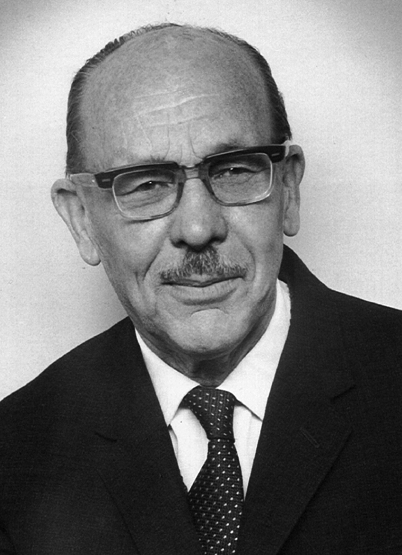
\includegraphics[height=4cm]{../images/KerrichBig.jpg}
\end{center}
\end{frame}

\begin{frame}{}

Fortunately Kerrich was imprisoned in a camp in Jutland run by the Danish Government in a `truly admirable way'. \\

\begin{center}
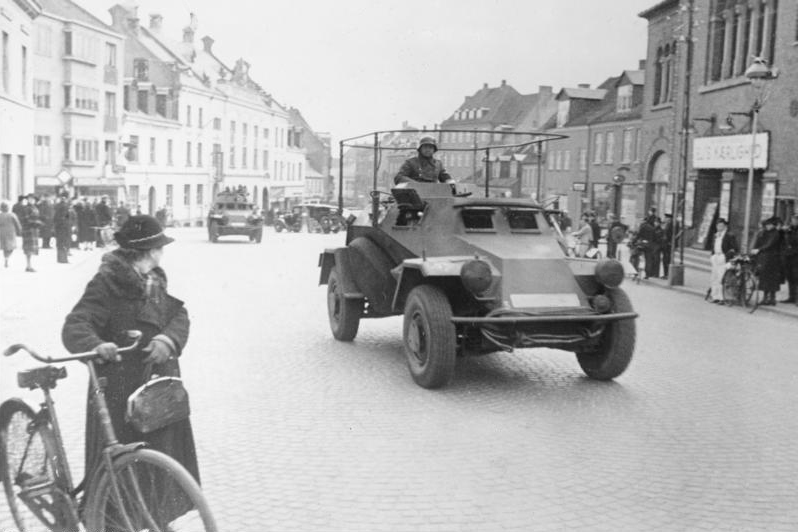
\includegraphics[height=5cm]{../images/Jutland.jpg}
\end{center}
\end{frame}

\begin{frame}{}

%'When Denmark was overrun by the Germans various British subjects were caught, Mr
%Kerrich among them. He was interned in a camp under Danish control
%and spent part of his enforced leisure in coin-tossing experiments' (Nature, 1946)

With a fellow internee Eric Christensen, Kerrich set up a sequence of experiments demonstrating the empirical validity of a number of fundamental laws of probability.

\begin{itemize}
\item They tossed a coin 10,000 times and counted the number of heads. \\
\item They made 5000 draws from a container with 4  ping pong balls (2x2 different brands), 'at the rate of 400 an hour, with - need it be stated - periods of rest between successive hours.'
\item They investigated tosses of a `biased coin', made from a wooden disk partly coated in lead.
\end{itemize}

In 1946 Kerrich published his finding in a monograph, {\it An
Experimental Introduction to the Theory of Probability}. 
\href{http://www.maths.usyd.edu.au/u/UG/JM/MATH1005/r/StatsData/Kerrich1950.pdf}{\beamergotobutton{Kerrich1950Paper}}

\vspace{.5cm}
{\bf How many heads do you think he counted? What is the probability of getting a head on a fair coin?}

\end{frame}

\subsection[]{Why study Probability?}
\begin{frame}{Why study Probability?}

Probability is often perceived as ‘scary’ because it conjures up impossible problems from School Maths Competitions! However ...

\begin{enumerate}
\item Probability is an essential part of every day life.  \\
 ``The most important questions of life ... are indeed for the most part only problems of probability."
 
 {\tiny (Laplace, {\it Théorie Analytique des Probabilitiés}, 1814)}
\href{http://bayes.wustl.edu/Manual/laplace_A_philosophical_essay_on_probabilities.pdf}{\beamergotobutton{Laplace1}}

\item 
Probability Theory makes many school problems easy. \\
``The theory of probabilities is basically just common sense reduced to calculus." 

{\tiny (Laplace, {\it Essai philosophique sur les probabilités},  1814)}
\href{http://archive.org/details/essaiphilosophiq00lapluoft}{\beamergotobutton{Laplace2}}

\item Probability (or the $p$-value) is crucial for decision making in Hypothesis Testing, which is essential to scientific research (Part 3).
\end{enumerate}
\end{frame}


\subsection[]{What is Probability?}
\begin{frame}{What is Probability?}

\begin{block}{Definition (Probability)}
The probability of an event is a measure of the likelihood of that event occurring. 
\end{block}

%Many systems are so complex that we rarely know the initial conditions accurately and so cannot predict outcomes (Newtonian physics).  Hence we adopt a stochastic viewpoint:  we identify the set of possible outcomes, and ascribe to each outcome (or set of outcomes) a probability $p  \in [0,1]$.

\vspace{.5cm}
Probability Theory is a set of mathematical tools which dates back centuries to casino type games. A more formal theory was developed in the 1930s by the Russian mathematician A. N. Kolmogorov.
\href{http://www.youtube.com/watch?v=2y3PH4SqmlA}{\beamergotobutton{History Video}}
\hyperlink{Appendix1}{\beamergotobutton{Appendix}}
\end{frame}

\subsection[]{Three types of Probability}
\begin{frame}{Three types of Probability}

{\bf (1) Subjective probability: based on belief} \\
The probability of an event is based on the strength of one’s belief.

\vspace{.5cm}
\begin{block}{Tossing a Fair Coin}
If I toss a fair coin once, the probability of getting a head is … 
\end{block}
\end{frame}


\begin{frame}{}

We rely on subjective probability for everyday decisions. But it can be abused.

\vspace{.5cm}
On March 27 1977 a PanAm 747 jet and a KLM 747 jet collided on an airport
runway in the Canary Islands killing 583 people.  Both jets had been scheduled for the Las Palmas Airport, but were diverted to Los Rodeos Airport (now called Tenerife) after  a group of militants set off a small bomb at the airport’s flower shop earlier that day. 

\begin{center}
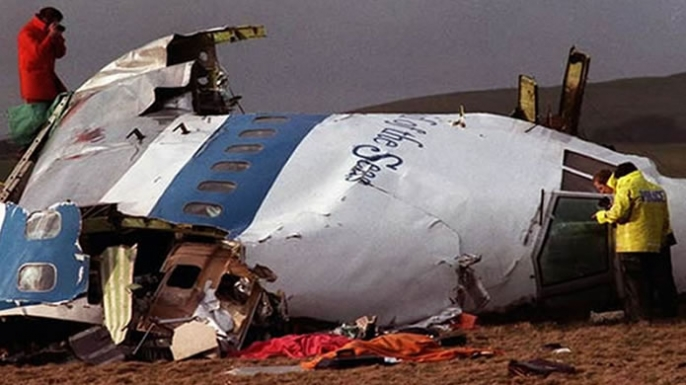
\includegraphics[height=3cm]{../images/Canary1.jpg}
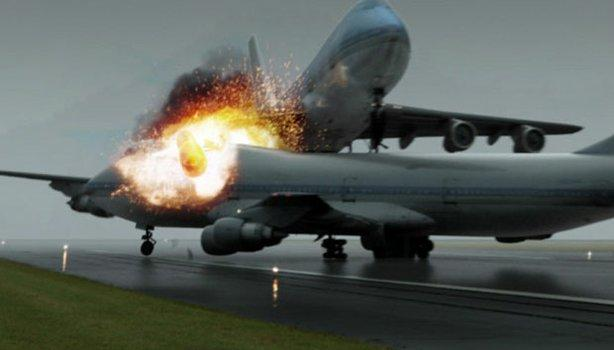
\includegraphics[height=3cm]{../images/Canary2Animation.jpg}
\end{center}
\end{frame}

\begin{frame}{}
The following statement was released: \\

\vspace{.5cm}
{\it NEW YORK, Mon: Mr. Webster Todd, Chairman
of the American National Transportation Safety Board
said today statistics showed that the chances of two
jumbo jets colliding on the ground were about 6 million
to one.} (AAP, quoted in West Australian, 1977)
\end{frame}


\begin{frame}{}
Australian statistician Terry Speed questioned the Chairman, with the following response: \\

\vspace{.5cm}
{\it Dear Professor Speed, \\
In response to your aerogram of April 5, 1977, the
Chairman’s statement concerning the chances of two
jumbo jets colliding (6 million to one) has no statistical
validity nor was it intended to be a rigorous or precise
probability statement. The statement was made to
emphasize the intuitive feeling that such an occurrence
indeed has a very remote but not impossible chance of
happening.
Thank you for your interest in this regard.}
\end{frame}



\begin{frame}{}

{\bf (2) Frequentist (or simulation) probability: based on data} \\
The probability of an event is the proportion of times that event would occur in a large number of repeated experiments (simulation).

\vspace{.5cm}
In some ways, subjective probability is an informal version of frequentist probability, using one's own history and experience (`personal data') as the basis.

\vspace{.5cm}
\begin{block}{Tossing a Fair Coin}
The probability of tossing a fair head =  $P(H)$ = The long run proportion of heads if we toss a fair coin a large number of times.
\end{block}
\end{frame}

\begin{frame}[fragile]{}

Famous Coin Tossers

\vspace{.5cm}
{\tiny \begin{tabular}{llll}
{\bf Person} & {\bf Number of Tosses} $n$ & {\bf Number of Heads} $x$ & $P(Head)$  \\  \hline
Count Buffon (1707-1788) 
\href{https://en.wikipedia.org/wiki/Georges-Louis_Leclerc,_Comte_de_Buffon}{\beamergotobutton{Buffon}}
& 4040 & 2048 & 0.507 \\ \hline
Karl Pearson (1857-1936) 
\href{https://en.wikipedia.org/wiki/Karl_Pearson}{\beamergotobutton{Pearson}}
& 24000 & 12012 & 0.5005 \\ \hline
John Kerrick (1903-1985 war camp) 
\href{https://en.wikipedia.org/wiki/John_Edmund_Kerrich}{\beamergotobutton{Kerrick}}
& 10000 & 5067 & 0.5067 \\ \hline
Perci Diaconis (1945-present) 
\href{http://statweb.stanford.edu/~susan/papers/headswithJ.pdf}{\beamergotobutton{Diaconis}}
& machine & & 0.51 \\ \hline
\end{tabular}}

\vspace{.5cm}
\begin{center}
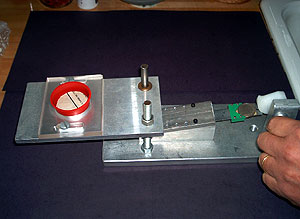
\includegraphics[height=4cm]{../images/CoinTosser.jpg}
\end{center}
\end{frame}

\begin{frame}[fragile]{}

In R Simulations

\begin{knitrout}
\definecolor{shadecolor}{rgb}{0.969, 0.969, 0.969}\color{fgcolor}\begin{kframe}
\begin{alltt}
\hlkwd{table}\hlstd{(}\hlkwd{sample}\hlstd{(}\hlkwd{c}\hlstd{(}\hlstr{"H"}\hlstd{,}\hlstr{"T"}\hlstd{),}\hlnum{4040}\hlstd{,}\hlkwc{replace}\hlstd{=T))}\hlopt{/}\hlnum{4040}
\end{alltt}
\begin{verbatim}
## 
##         H         T 
## 0.4933168 0.5066832
\end{verbatim}
\begin{alltt}
\hlkwd{table}\hlstd{(}\hlkwd{sample}\hlstd{(}\hlkwd{c}\hlstd{(}\hlstr{"H"}\hlstd{,}\hlstr{"T"}\hlstd{),}\hlnum{24000}\hlstd{,T))}\hlopt{/}\hlnum{24000}
\end{alltt}
\begin{verbatim}
## 
##         H         T 
## 0.5015833 0.4984167
\end{verbatim}
\begin{alltt}
\hlkwd{table}\hlstd{(}\hlkwd{sample}\hlstd{(}\hlkwd{c}\hlstd{(}\hlstr{"H"}\hlstd{,}\hlstr{"T"}\hlstd{),}\hlnum{10000}\hlstd{,T))}\hlopt{/}\hlnum{10000}
\end{alltt}
\begin{verbatim}
## 
##     H     T 
## 0.503 0.497
\end{verbatim}
\end{kframe}
\end{knitrout}

\end{frame}

\begin{frame}{}
Kerrich's Tosses: Proportion of Heads
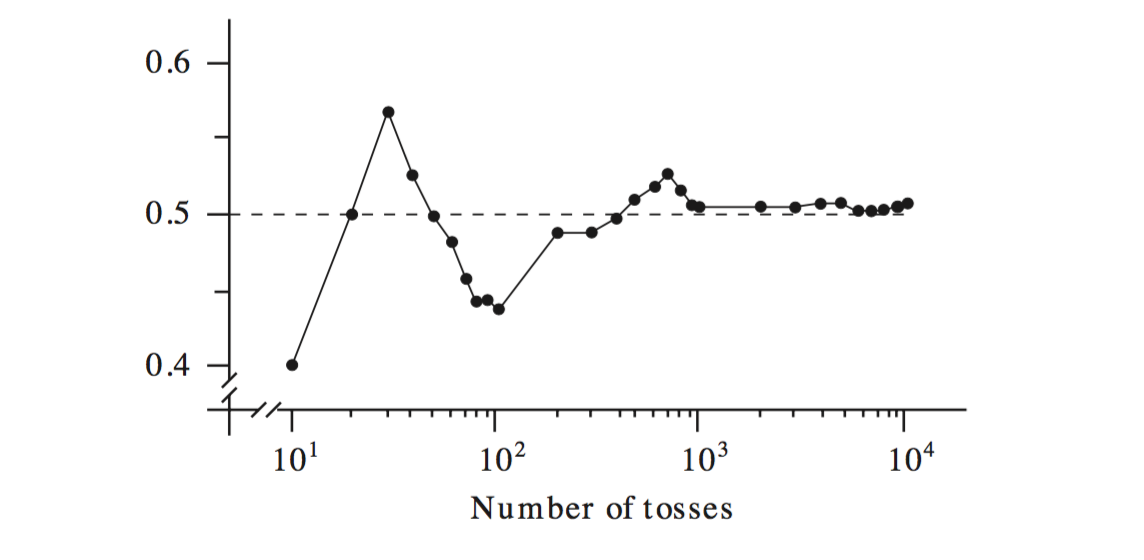
\includegraphics[height=6cm]{../images/KerrichTosses.jpg}

This illustrates the `Law of Averages' or `Law of Large Numbers': the proportion of heads becomes more stable as the length of the simulation increases and approaches a fixed number called the `relative frequency'.

\end{frame}


\begin{frame}{}

{\bf (3) Theoretical (or classical) probability: based on model} \\
The probability of an event is based on a model of the context. 

\vspace{.5cm}
Two models for Coin Tossing: 

\vspace{.5cm}
(1) Physics model: the side that the coin lands on is determined by a number of complicated factors such as which way up it started, the degree of spin, the speed and angle with which it left the thumb and how far it has to fall.
\href{https://www.youtube.com/watch?v=AYnJv68T3MM}{\beamergotobutton{PercisDiaconisVideo1}} 
\href{https://www.youtube.com/watch?v=Obg7JPd6cmw}{\beamergotobutton{PercisDiaconisVideo2}}

\begin{center}
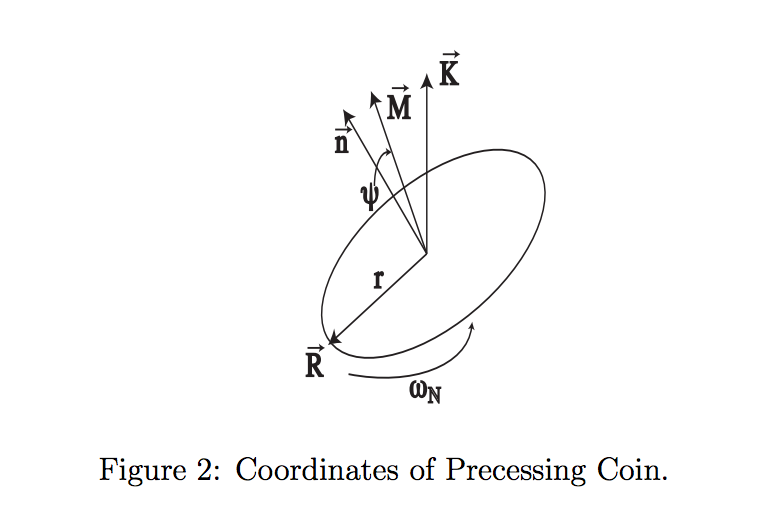
\includegraphics[height=3cm]{../images/CoinPhysics.jpg}
\end{center}

\end{frame}

\begin{frame}{}

(2) Standard model: Tossing a fair coin results in a head and a tail half the time, in an unpredictable order (random). 

\vspace{.5cm}
\begin{block}{Tossing a Fair Coin}
Given a coin toss has 2 outcomes, the probability of tossing a fair head =  $\frac{1}{2}$.
\end{block}

\vspace{.5cm}
This is the model used for decisions in sport (eg which team starts with the ball in AFL, or which team bats or bowls first in cricket).

\begin{center}
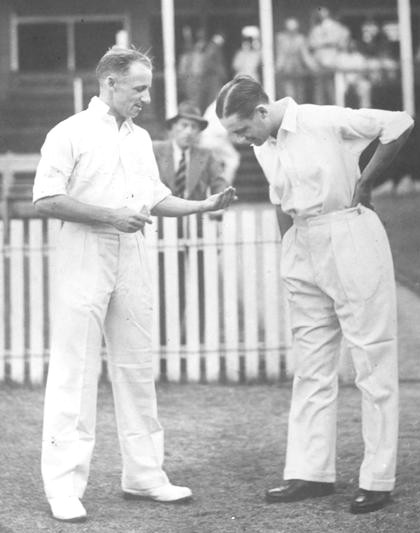
\includegraphics[height=3cm]{../images/BradmanAllenToss.jpg}
\end{center}

\vspace{.5cm}
{\tiny Note: In later Stats courses, you will also learn about Bayesian Probability.}

\end{frame}


\begin{frame}[fragile]{}
\begin{alertblock}{Extension}
Suppose you toss a fair coin 1000 times:  when it lands heads
you receive \$1, and when it lands tails you pay me \$1.
What is your expected profit or loss?
\end{alertblock}

Using Simulation:
\begin{knitrout}
\definecolor{shadecolor}{rgb}{0.969, 0.969, 0.969}\color{fgcolor}\begin{kframe}
\begin{alltt}
\hlkwd{set.seed}\hlstd{(}\hlnum{1}\hlstd{)}
\hlstd{CoinTosses} \hlkwb{<-} \hlkwd{sample}\hlstd{(}\hlkwd{c}\hlstd{(}\hlopt{-}\hlnum{1}\hlstd{,}\hlnum{1}\hlstd{),} \hlnum{1000}\hlstd{,} \hlkwc{replace} \hlstd{=} \hlnum{TRUE}\hlstd{)}
\hlkwd{plot}\hlstd{(}\hlkwd{cumsum}\hlstd{(CoinTosses),}\hlkwc{xlab}\hlstd{=}\hlstr{"Tosses"}\hlstd{,} \hlkwc{ylab}\hlstd{=}\hlstr{"P/L"}\hlstd{,} \hlkwc{type}\hlstd{=}\hlstr{"l"}\hlstd{)}
\end{alltt}
\end{kframe}
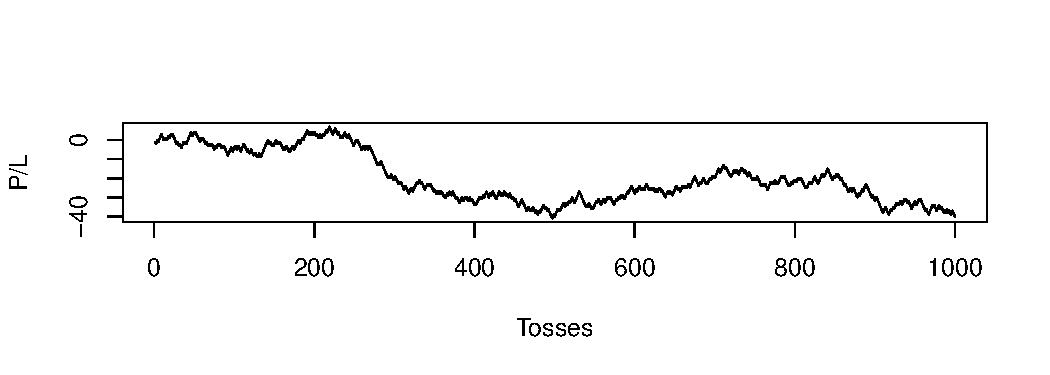
\includegraphics[width=\maxwidth]{figure/unnamed-chunk-3-1} 

\end{knitrout}
\end{frame}


\begin{frame}{}
We could run this simulation 10000 times, resulting in:

\begin{knitrout}
\definecolor{shadecolor}{rgb}{0.969, 0.969, 0.969}\color{fgcolor}
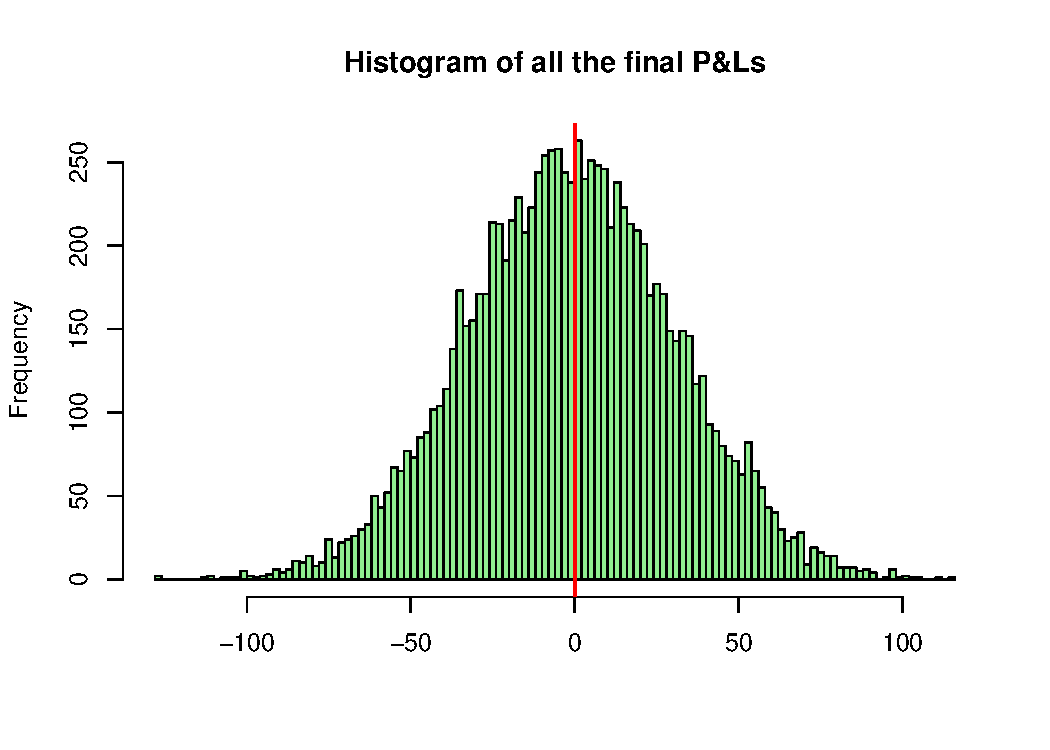
\includegraphics[width=\maxwidth]{figure/unnamed-chunk-4-1} 

\end{knitrout}

In Topic 5, we will see how to solve this theoretically.

\end{frame}


\subsection[]{Describing Simple Probability Models}

\begin{frame}[fragile]{Describing Simple Probability Models}
We can describe simple probability models using set notation and the Venn diagram.

\vspace{.5cm}
\begin{tabular}{lll}
Symbol & Name & Meaning \\ \hline
$\Omega$ & Sample Space & Everything that can occur. \\
$A, B, \ldots$ & Events & A subset of the sample space. \\ $\emptyset$  & Empty Set & An event which cannot occur. \\
 $A^{'}$ or $A^c$ & Complement & Everything not in $A$. \\
$A \subset \Omega$  & Belongs to & Event A belongs to sample space $\Omega$. \\
\end{tabular}

\begin{center}
\begin{tikzpicture}
\draw (-3,-1.5) rectangle (3,1.5) node[below left]{$\Omega$}
 node[below right]{$A \subset \Omega$};
\fill[green] (0,0) circle (1cm);
\draw (0,0) circle (1cm) node {$A$};
\end{tikzpicture}
\end{center}

\end{frame}


\begin{frame}[fragile]{}

{\bf If $A$ and $B$ $\subset \Omega$:} 

\vspace{.5cm}
\begin{tabular}{lll}
Symbol & Name & Meaning \\ \hline
$A \cup B$ & Union & $A$ or $B$ or both occur. \\
$A \cap B$ & Intersection & Both $A$ and $B$ occur. \\
$A  \setminus B$ & Minus or Relative Complement & In $A$ but  not in $B$. \\
\end{tabular}

%% Picture of A Union B
\vspace{1cm}
\begin{center}
\begin{tikzpicture}
\draw (-2,-1.5) rectangle (3.5,1.5) node[below left]{$\Omega$}  node[below right]{$A \cup B $};
\fill[green] (0,0) circle (1cm);
\fill[green] (1.5,0) circle (1cm);
\draw (0,0) circle (1cm) node {$A$};
\draw (1.5,0) circle (1cm) node {$B$};
\end{tikzpicture}
\end{center}
\end{frame}

%% Picture of A Intersection B
\begin{frame}
\begin{center}
\begin{tikzpicture}
\draw (-2,-1.5) rectangle (3.5,1.5) node[below left]{$\Omega$} node[below right]{$A \cap B $};
\begin{scope} % start of clip scope
\clip (0,0) circle (1cm);   % keep only what is inside A
\fill[green] (1.5,0) circle (1cm);   % draw region B
\end{scope} % end of clip scope
\draw (0,0) circle (1cm) node[left] {$A$};
\draw (1.5,0) circle (1cm) node[right] {$B$};
\end{tikzpicture}
\end{center}

%% Picture of A Minus B
\begin{center}
\begin{tikzpicture}
\draw (-2,-1.5) rectangle (3.5,1.5) node[below left]{$\Omega$} node[below right]{$A \setminus B $};
\begin{scope}{even odd rule} % start of clip scope
\clip (1.5,0) circle (1cm) (-2,-1.5) rectangle (3.5,1.5);   % complement of B
\fill[green] (0,0) circle (1cm);   % draw region A
\end{scope} % end of clip scope
\draw (0,0) circle (1cm) node[left] {$A$};
\draw (1.5,0) circle (1cm) node[right] {$B$};
\end{tikzpicture}
\end{center}
\end{frame}



\begin{frame}[fragile]{}
\vspace{.5cm}
{\bf If $A_{1}, A_{2}, \ldots \subset \Omega$:} 

\vspace{.5cm}
\begin{tabular}{lll}
Symbol & Name & Meaning \\ \hline
$\cup A_{i=1}^{n}$ & Union & One or more of $A_{i}$ occur. \\
$\cap A_{i=1}^{n}$ & Intersection & All $A_{i}$ occur. \\
\end{tabular}
\end{frame}


\begin{frame}{Example}
\begin{alertblock}{Your Turn (Set Notation)}
Describe the grey and white regions in set notation.
% Grey = $A \cap B \cap C'$; White = $ A \cap B \cap C$
\begin{center}
\begin{tikzpicture}
\draw \setO node[below left]{$\Omega$};
\begin{scope}
\clip \setA;
\fill[gray] \setB;
\end{scope}
\begin{scope}
\clip \setA;
\clip \setB;
\fill[white] \setC;
\end{scope}
\draw \setA node[left] {$A$};
\draw \setB node[right] {$B$};
\draw \setC node {$C$};
\end{tikzpicture}
\end{center}
\end{alertblock}
\end{frame}


\begin{frame}{}
\begin{alertblock}{Your Turn (Sample Space)}
\begin{itemize}

\item A coin is tossed to start a cricket match. What is the probability of landing on its edge? \\

\item For the following scenarios, what is $\Omega$?

\begin{itemize} 
\item A coin is tossed until a head occurs. 
\item The 2016 Australian census question about Gender.
\item Measuring tomorrow's rainfall.
\end{itemize}
\end{itemize}

\end{alertblock}
\end{frame}


\subsection[]{Probability Results}
\begin{frame}[fragile]{Probability Results}

\begin{itemize}
\item 
Classical Probability \\
Where the sample space $\Omega$ consist of a finite, known number of equally likely outcomes (eg coins, dice, cards), 
the probability of an event $A \subset \Omega$ occurring is 

\[\boxed{ P(A) = \frac{\mbox{Number of ways $A$ can occur}}{\mbox{Total number of possible outcomes in } \Omega} }  \] 

\vspace{.5cm}
where \\
$P(A) = 0$ (impossible event)  \\
$P(A) = 1$ (certain event) \\
\end{itemize}
\end{frame}
 
\begin{frame}\frametitle{}  
\begin{itemize}
\item
Complement \\
The probability that an event $A$ does not occur is

\[ \boxed{ P(A') = 1 - P(A)  }\]

\vspace{.5cm}
\item Mutually Exclusive \\
2 events $A$ and $B$ are mutually exclusive if
\[ \boxed{ P(A \cap B) = 0 } \]

\vspace{.25cm}
%% Picture of Mutually Exclusive
\begin{center}
\begin{tikzpicture}
\draw (-2,-1.5) rectangle (6,1.5) node[below left]{$\Omega$}  node[below right]{};
\draw (0,0) circle (1cm) node {$A$};
\draw (3,0) circle (1cm) node {$B$};
\end{tikzpicture}
\end{center}
\end{itemize}

Note: This is not a 'rule' but a definition. We position it here, to see comparison with independence.
\end{frame} 


\begin{frame}[label=Setindependence]\frametitle{} 
\begin{itemize}
\item Independence \\
2 events $A$ and $B$ are independent (the result of one does not affect the result of the other) iff

\[ \boxed{ P(A \cap B) = P(A)P(B)  }\]

\vspace{.5cm}
%% Picture of Independent Events
\begin{center}
\begin{tikzpicture}
\draw (-2,-1.5) rectangle (3.5,1.5) node[below left]{$\Omega$} node[below right]{\tiny{$P(A)=0.2$, $P(B)=0.5$, $P(A \cap B) = 0.1$}};
\begin{scope} % start of clip scope
\clip (0,0) circle (1cm);   % keep only what is inside A
\fill[green] (1.5,0) circle (1cm);   % draw region B
\end{scope} % end of clip scope
\draw (0,0) circle (1cm) node[left] {$A$};
\draw (1.5,0) circle (1cm) node[right] {$B$};
\end{tikzpicture}
\end{center}
\end{itemize}
\end{frame}
 
\begin{frame}\frametitle{} 
\begin{itemize}

\item Union Rule \\
For events $A$ and $B \subset \Omega$, then 

\[ \boxed{ P(A \cup B) = P(A) + P(B) – P(A \cap B) } \]

\vspace{.5cm}
%% Picture of A Union B
\begin{center}
\begin{tikzpicture}
\draw (-2,-1.5) rectangle (3.5,1.5) node[below left]{$\Omega$}  node[below right]{};
\fill[green] (0,0) circle (1cm);
\fill[green] (1.5,0) circle (1cm);
\draw (0,0) circle (1cm) node {$A$};
\draw (1.5,0) circle (1cm) node {$B$};
\end{tikzpicture}
\end{center}
\end{itemize}
\end{frame}

\begin{frame}{}

For mutually exclusive events, this reduces to

\[ \boxed{ P(A \cup B) = P(A) + P(B) } \]

\vspace{.5cm}
%% Picture of A Union B
\begin{center}
\begin{tikzpicture}
\draw (-2,-1.5) rectangle (5,1.5) node[below left]{$\Omega$}  node[below right]{};
\fill[green] (0,0) circle (1cm);
\fill[green] (2.5,0) circle (1cm);
\draw (0,0) circle (1cm) node {$A$};
\draw (2.5,0) circle (1cm) node {$B$};
\end{tikzpicture}
\end{center}
\end{frame}
 
\begin{frame}\frametitle{} 
\begin{itemize}

\item Conditional Probability \\
For events $A$ and $B \subset \Omega$ where $P(B) \neq 0$, the conditional probability of $A$ given $B$ is

\[  \boxed{ P(A | B) = \frac{ P(A \cap B)}{P(B)} } \]

\vspace{.5cm}
This leads to a second definition of independence:

2 events $A$ and $B$ are independent iff

\[ \boxed{ P(A | B) = P(A)  }\]

\end{itemize}
\end{frame}

\begin{frame}\frametitle{} 
\begin{itemize}

\item Bayes Theorem

\[  \boxed{ P(A | B) = \frac{ P(B | A) P(A)}{P(B)} } \]

\href{https://en.wikipedia.org/wiki/Confusion_of_the_inverse}{\beamergotobutton{Bayes Theorem}}

\vspace{.5cm}
\item The Law of Total Probability
 
 \[ \boxed{  P(A) = \sum_{i}^{} P(A | B_{i}) P(B_{i}) } \]
 
 for any $i$ for which $P(B_{i}) \neq 0$.

\end{itemize}
\end{frame}

\subsection[]{Counting Short Cuts}
\begin{frame}[label=Factorials]{Counting Short Cuts}
\frametitle{} 

Computing classical probabilities amounts to careful counting, so we have the following short-cuts.

\vspace{.5cm}
\begin{block}{Multiplication Principle for $k$ stage problems}
If an experiment consists of $k$ stages where the $i$th stage has $n_{i}$ outcomes (for $i=1,2,\ldots k$), then the total number of outcomes is $n_{1} n_{2} \ldots n_{k}$.
\end{block}

\vspace{.5cm}
\begin{block}{Definition (Permutations, Factorials)}
Any $x$ distinct objects can be permuted (or rearranged) in $x! = x(x-1)(x-2) \ldots 3 2 1$ ways.
\end{block}
\end{frame}

\begin{frame}[label=BinomialCoefficients,fragile]
\frametitle{} 

\begin{block}{Definition (Combinations, Binomial Coefficients)}
The number of ways of choosing a group of $x$ objects from $n$ objects is 
\[ {n \choose x}  = \frac{n!}{x! (n-x)!} \]
where by definition $0! = 1$.
\end{block}

\begin{knitrout}
\definecolor{shadecolor}{rgb}{0.969, 0.969, 0.969}\color{fgcolor}\begin{kframe}
\begin{alltt}
\hlkwd{factorial}\hlstd{(}\hlnum{10}\hlstd{)}\hlopt{/}\hlstd{(}\hlkwd{factorial}\hlstd{(}\hlnum{8}\hlstd{)}\hlopt{*}\hlkwd{factorial}\hlstd{(}\hlnum{2}\hlstd{))}
\end{alltt}
\begin{verbatim}
## [1] 45
\end{verbatim}
\begin{alltt}
\hlkwd{choose}\hlstd{(}\hlnum{10}\hlstd{,}\hlnum{2}\hlstd{)}
\end{alltt}
\begin{verbatim}
## [1] 45
\end{verbatim}
\end{kframe}
\end{knitrout}
\end{frame}
 
\begin{frame}{Examples}
\begin{alertblock}{Your Turn}
\begin{itemize}
\item Suppose a mobile phone number of length 10 starts with the numbers 04.  How many unique numbers can be issued?  Assuming all numbers are randomly issued, what is the probability of getting the number $04********$, where $*$ = 0,1, ... 9.  \\

\item A chain is formed from $n$ independent links, with a probability of $\theta$ that any link fails under a  specified load. What is the probability that the chain fails under the load? 

\item The probability that a component lasts at least $x$ hours is $e^{-x/100}$, for $x > 0$. What is the probability  that the component lasts at least 10 hours, given it has already lasted at least 6 hours? 
\end{itemize}
\end{alertblock}
\end{frame}

\subsection[]{Random Variables}
\begin{frame}{Why Random Variables?}

\begin{block}{Definition (Random Variable)}
A random variable is a real valued function on a sample space $\Omega$, that 
captures both the outcomes and associated probabilities.
\end{block}

A random variable is a simple way of summarising a probability problem. It sharpens our focus by summarising the outcomes and highlighting the events of interest. 

\vspace{.5cm}
We use a capital Roman letter $X$ to denote a random variable and the corresponding lower case letter $x$ to denote the values of the random variable. We will consider discrete and continuous random variables, depending on the underlying context.
\end{frame}

\begin{frame}[fragile]{Examples}
\begin{alertblock}{Your Turn}
Consider the following 3 functions. Is $X$ a random variable?

\begin{center}
\begin{tabular}{|l|l|l|l|l|} \hline
$x$ & -1 & 0 & 1 & Total \\ \hline
$f(x)$ & -0.2 & 1 & 0.2 & \\ \hline
\end{tabular}
\end{center}

\begin{center}
\begin{tabular}{|l|l|l|l|l|} \hline
$x$ & -1 & 0 & 1 & Total \\ \hline
$f(x)$ & 0.4 & 0.2 & 0.3 & \\ \hline
\end{tabular}
\end{center}

\begin{center}
\begin{tabular}{|l|l|l|l|l|} \hline
$x$ & -1 & 0 & 1 & Total \\ \hline
$f(x)$ & 0.4 & 0.3 & 0.3 & \\ \hline
\end{tabular}
\end{center}
\end{alertblock}
\end{frame}

\begin{frame}{}
\begin{block}{Coin Tossing 5 times}
Toss a fair coin 5 times. What is the probability of getting 4 or more heads?

\vspace{.5cm}
{\bf Long way: List Sample Space}  \\
$ \Omega = 
\{  HHHHH, \ldots, TTTTT\} , |\Omega| = 2^5 = 32$ \\
$ P( \mbox{4 or more heads})  =  \frac{6}{32} = \frac{3}{16}$ 

\vspace{.5cm}
{\bf Neater way: Summarise by defining a random variable} \\
Let $X = $ the number of heads in 5 tosses of a coin, $x=0,1,\ldots,5$.

\begin{center}
\begin{tabular}{|l|l|l|l|l|l|l|} \hline
$x$ & 0 & 1 & 2 & 3 & 4 & 5  \\ \hline
$P(X=x)$ & $\frac{1}{32}$ & $\frac{5}{32}$ & $\frac{10}{32}$ & $\frac{10}{32}$ & $\frac{5}{32}$ & $\frac{1}{32}$  \\ \hline
\end{tabular}
\end{center}

\[P( X \geq 4)  =  \frac{6}{32}   \]

\end{block}
\end{frame}

\begin{frame}{}
\begin{block}{Your Turn (Die)}
Toss a fair die 2 times. What is the probability of getting a total of 8 or more?

\vspace{.5cm}
{\bf Long way: List Sample Space} \\
\[ \Omega = 
\{  \begin{tabular}{l}
11,12,13,14,15,16 \\
21,22,23.24.25.26 \\
31,32,33,34,35,36 \\
41,42,43,44,45,46 \\
51,52,53,54,55,56 \\
61,62,63,64,65,66
\end{tabular}
\} , |\Omega| = 36 \]

\[P( \mbox{Total of 8 or more})  =  \frac{15}{36}   \]

\end{block}
\end{frame}

\begin{frame}[fragile]{}
\begin{block}{}

{\bf Neater way: Summarise by defining a random variable} \\
Let $X = $ the total of 2 tosses of a die, $x=2,3,\ldots,12$.

\begin{center}
\begin{tabular}{|l|l|l|l|l|l|l|l|l|l|l|l|} \hline
$x$ & 2 & 3 & 4 & 5 & 6 & 7 & 8 & 9 & 10 & 11 & 12  \\ \hline
$P(X=x)$ & $\frac{1}{36}$ & $\frac{2}{36}$ & $\frac{3}{36}$ & $\frac{4}{36}$ & $\frac{5}{36}$ & $\frac{6}{36}$ & $\frac{5}{36}$ & $\frac{4}{36}$ & $\frac{3}{36}$ & $\frac{2}{36}$ & $\frac{1}{36}$  \\ \hline
\end{tabular}
\end{center}

\[P( X \geq 8)  =  \frac{15}{36}   \]

\end{block}
\end{frame}

\subsection[Distributions]{Distributions}
\begin{frame}\frametitle{What is a Distribution?}
\begin{definition}[Distribution]
A \alert{distribution} defines the behaviour of a situation modelled by a variable $X$, in particular
\begin{itemize}
\item the set of all possible values $\{ x \}$ \\
"what can happen"

\item the probability of each value (discrete) or each range of values (continuous) occuring.\\
"how often everything happens"
\end{itemize}

\end{definition}
\end{frame}

\begin{frame}[fragile, label=CDF]\frametitle{Probability Functions}

\begin{definition}[Probability Functions]

For a variable $X$, we can describe the probabilities by:
\begin{itemize}
\item the \alert{probability distribution function} (for discrete variables) \\ 
$P(X=x)$

\item  the \alert{probability density function (pdf)} (for continuous variables) \\  $f(x)$ \\
\item  the \alert{cumulative distribution function (CDF)} (for both discrete and continuous variables)  \\
$F(x) = P(X \leq x)$

\end{itemize}
\end{definition}
\end{frame}

\begin{frame}\frametitle{Types of Distributions}

\begin{definition}[Types of Distributions]
We can characterise distributions in 2 ways:

\vspace{.5cm}
By \alert{context}:
\begin{itemize}
\item population distribution
\item sample distribution
\item sampling distribution (for a statistic like $\bar{X}$).
\end{itemize}

\vspace{.5cm}
By \alert{underlying nature}:
\begin{itemize}
\item discrete distribution 
\item continuous distributions
\end{itemize}
\end{definition}
\end{frame}

\begin{frame}\frametitle{Notes on Distributions}
\begin{itemize}
\item
The distribution can be referred to as the {\it probability} distribution or the {\it statistical} distribution.
\item The sample distribution can suggest the population distribution, especially for large sample size $n$. 
\item For a population distribution, the mean is $\mu$ and the variance is $\sigma^2$. For a sample distribution, the mean is $\bar{x}$ and the variance is $s^2$.
\end{itemize}

\vspace{.5cm}
\begin{tabular}{l|l|l}
 & Population: Parameter & Sample: Statistic \\ \hline
Mean & $\mu$ & $\bar{x}$ \\ \hline
Standard Deviation & $\sigma$ & $s$ \\ \hline
\end{tabular}


\end{frame}
\end{document}
